%---
\section{The \dsf\ Detectors}
\label{sec:detector}

The \dsf\ apparatus consists of three nested detectors, see Fig.~\ref{fig:ds-50-detectors}.  From the center outward, the three detectors are: the Liquid Argon Time Projection Chamber, which is the dark matter detector; the Liquid Scintillator Veto (\lsv), serving as shielding and as anti-coincidence for radiogenic and cosmogenic neutrons, {\gr s}, and cosmic muons; and the Water Cherenkov Detector (\wcd), serving as shielding and as anti-coincidence for cosmic muons~\cite{ctf:results,ctf:scitech}.  The detector system is located in Hall C of LNGS at a depth of \lngsequivdepth\ \cite{lngs-depth}, in close proximity to and sharing many facilities with, the Borexino solar neutrino detector~\cite{bx:detector,bx:plants}.  

The \lar\ \tpc\ can exploit pulse shape discrimination and the ratio of scintillation to ionization to reject \bg\ background in favor of the nuclear recoil events expected from WIMP scattering~\cite{boulay,warp}.  It can also exploit the \tpc's spatial resolution to reject surface backgrounds and to reject multi-sited events.  Events due to neutrons from cosmogenic sources and from radioactive contamination in the detector components, which also produce nuclear recoils, are suppressed by the combined action of the neutron and cosmic ray vetoes.  The liquid scintillator also provides additional rejection of $\gamma$-ray background from the detector materials.  The water-plus-liquid scintillator design was motivated in part by the success of this shielding concept in achieving very low backgrounds in Borexino~\cite{bx:detector,bx:7be-precision,bx:phase-I}.

The \wcd\ is an \ctfdiameter-diameter, \ctfheight-high cylindrical tank filled with high purity water.  The tank was originally part of the Borexino Counting Test Facility.  The inside surface of the tank is covered with a laminated Tyvek-polyethylene-Tyvek reflector~\cite{daya-bay}.  An array of \ctfpmtnum\ \ctfpmt\ \ctfpmtsize~{\pmt s}, with \ctfpmtqe\ average quantum efficiency (QE) at \ctfpmtwave, is mounted on the side and bottom of the water tank to detect Cherenkov photons produced by muons or other relativistic particles traversing the water.

The \lsv\ is a \lsvdiameter-diameter stainless steel sphere filled with \lsvscintillatormass\ of borated liquid scintillator.  The scintillator consists of equal amounts of pseudocumene (PC) and trimethyl borate (TMB), with the wavelength shifter Diphenyloxazole (PPO) at a concentration of \lsvppoconcentration.  The sphere is lined with Lumirror~\cite{lumirror} reflecting foils.  An array of  \lsvpmtnum\ \lsvpmt\ \lsvpmtsize~{\pmt s}, with low-radioactivity glass bulbs and high-quantum-efficiency photocathodes (\lsvpmtqe\ average QE at \lsvpmtwave), is mounted on the inside surface of the sphere to detect scintillation photons.

The neutron-capture reaction \borten($n$,$\alpha$)\lith\ makes the borated scintillator a very effective veto of neutron background~\cite{wright}.   The \tmb, \tmbchem, contains $^{\rm nat}$B which has a \abborten\ natural abundance of \borten\ with its large (\lsvbtenxsec) thermal neutron capture cross section.  The thermal neutron capture time in the borated scintillator is calculated to be just \lsvtmbfiftypercentcapturetime, compared to \lsvtmbzeropercentcapturetime\ for pure \pc~\cite{bx:detector}.  


The \borten\ neutron capture proceeds to the \lith\ ground state with branching ratio \brbortenground, producing a \enbortengroundalpha\ $\alpha$ particle, and to a \lith\ excited state with branching ratio \brbortenexcited\, producing a \enbortenexcitedalpha\ $\alpha$ particle and a gamma-ray of \enbortenexcitedgamma.  Because of quenching, the scintillation light output of the capture to \lith(g.s.) is expected to be in the \bg-equivalent range \lsvalphaequivenergy~\cite{greenwood,wang}.  
Preliminary measurements with our scintillator appear consistent with this expectation.
The measured \lsv\ photoelectron (\si{\pe}) yield is \lsvly, making this quenched energy readily detectable.  The high \cfor\ decay rate in the \lsv\ and the fact that its spectrum covers the signal expected from the $\alpha$'s from neutron capture on \borten\ severely reduced the effectiveness of the neutron veto in the present data set.  The rejection power is estimated from simulations to be \odneutronrejectionachieved\ instead of the design value of~\odneutronrejectiondesign~\cite{wright}.

\begin{figure}[t!]
\begin{center}
\includegraphics[height=0.7\columnwidth]{Figures/ds-50-assembly.jpg}
\caption{The nested detector system of \dsf. The outermost gray cylinder is the \wcd, the sphere is the \lsv, and the gray cylinder at the center of the sphere is the \lar\ \tpc\ cryostat.}
\label{fig:ds-50-detectors}
\end{center}
\end{figure}

The \dsf\ \tpc, as shown in Fig.~\ref{fig:ds-50-detectors}, is contained in a stainless steel cryostat that is supported at  the center of the \lsv\ on a system of leveling rods.  Its design was based on that of the \dst\ prototype, which operated for \dstexp\ at LNGS~\cite{ds:ds-10-run3}. 
A cut-away view of of the \tpc\ is given in Fig.~\ref{fig:ds-50-tpc}.

Ionizing events in the active volume of the \lar\ \tpc\ result in a prompt scintillation signal called ``\sone''.  Ionization electrons escaping recombination drift in the \tpc\ electric field to the surface of the \lar, where a stronger electric field extracts them into an argon gas layer between the \lar\ surface and the \tpc\ anode.  The electric field in the gas is large enough to accelerate the electrons so that they excite the argon, resulting in a secondary scintillation signal, ``\stwo'', proportional to the collected ionization.  Both the scintillation signal \sone\ and the ionization signal \stwo\ are measured by the same \pmt\ array.  The temporal pulse shape of the \sone\ signal provides discrimination between nuclear-recoil and electron-recoil events.  The \stwo\ signal allows the three-dimensional position of the energy deposition to be determined and, in combination with \sone, provides further discrimination of signal from background.   A significant fraction of events also exhibit an ``\sthree" signal.  The S3 pulse resembles \stwo\ in pulse shape but is typically \dsfstwooversthree\ times smaller and always follows \stwo\ by a fixed delay equal to the maximum drift time in the \lar\ \tpc.  \sthree\ is believed to result from electrons released from the cathode (at the bottom of the TPC) when struck by the bright \stwo\ UV light.

\begin{figure}[t!]
\begin{center}
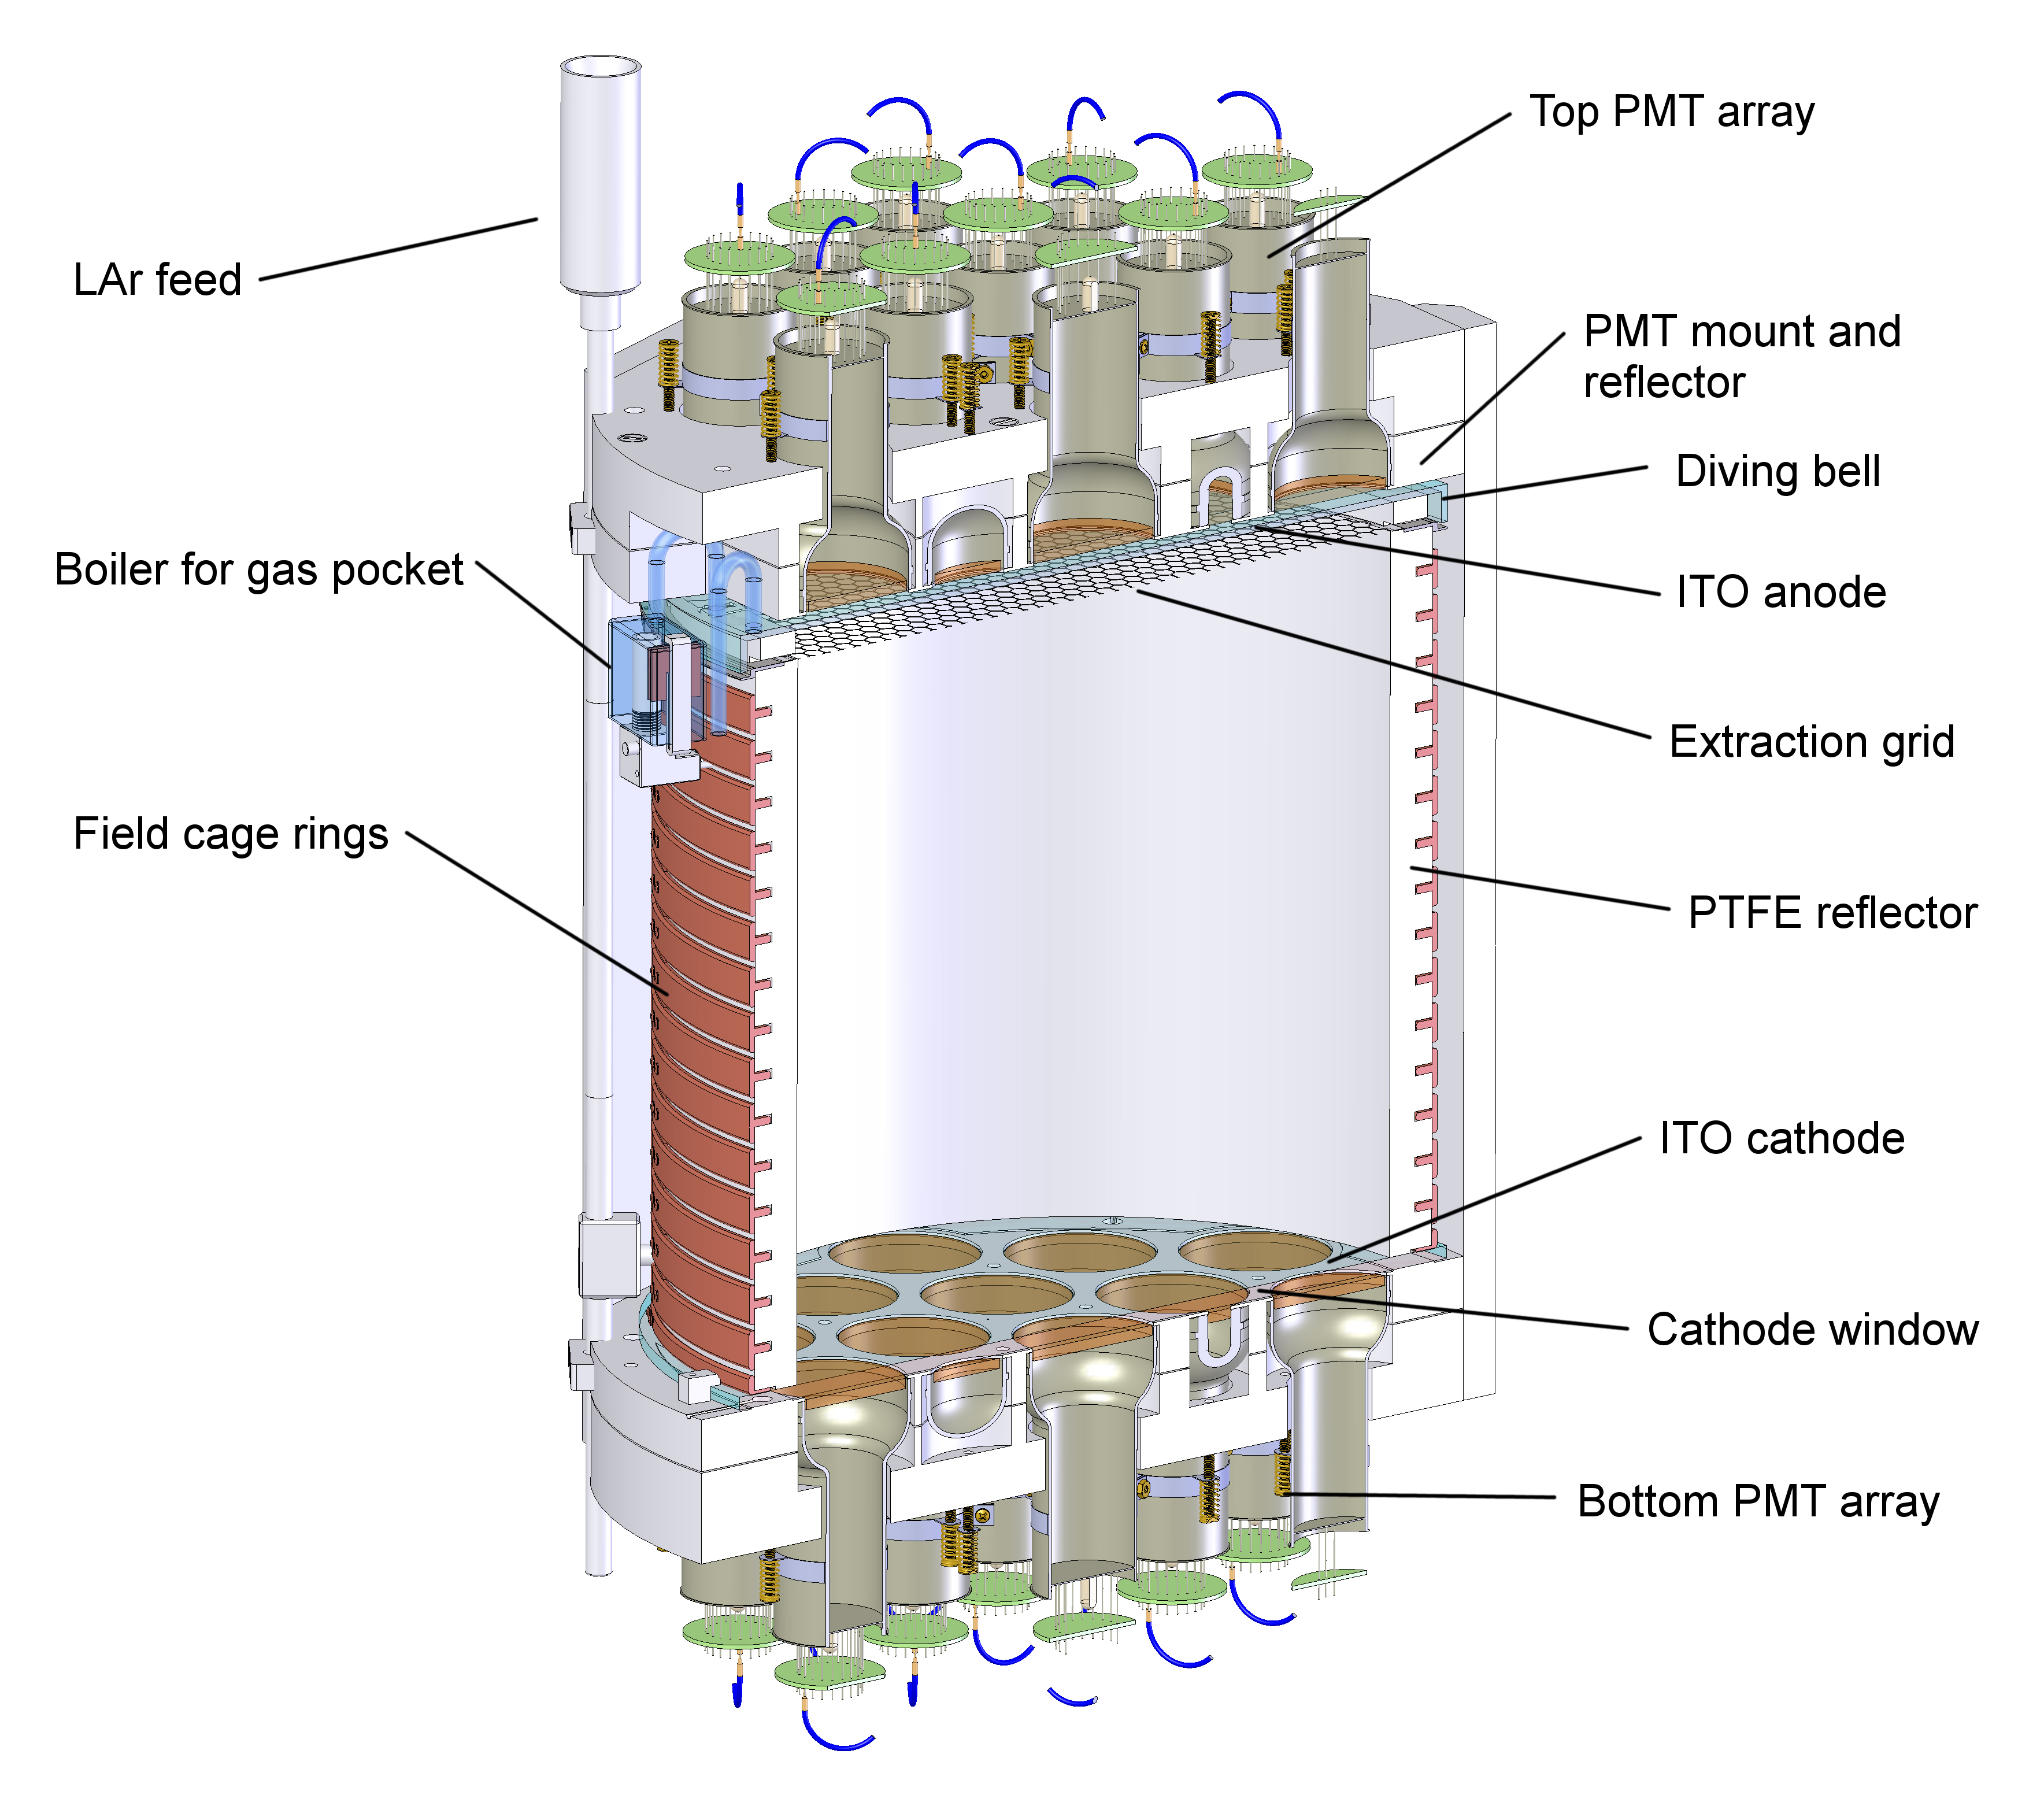
\includegraphics[height=4.0in]{Figures/50kg_Assembly_4-1-13_section_annotated_2.JPG}
\caption{The \dsf\ Liquid Argon Time Projection Chamber.}
\label{fig:ds-50-tpc}
\end{center}
\end{figure}

The active \lar\ is contained in a cylindrical region viewed by \dsfpmtnum\ \dsfpmt\ \dsfpmtsize\ low-background, high-quantum-efficiency  {\pmt s}, nineteen each on the top and the bottom.  The average quantum efficiency of the {\pmt s} at room temperature is \dsfpmtqe\ at \dsfpmtwave.  The  {\pmt s} are submerged in liquid argon and view the active \lar\ through fused-silica windows, which are coated on both faces with transparent conductive indium tin oxide (\ito) films \dsfitothickness\ thick.  This allows the inner window faces to serve as the grounded anode (top) and $-$HV cathode (bottom) of the \tpc\ while maintaining their outer faces at the average \pmt\ photocathode potential.  The cylindrical wall is a \dsfthickptfereplector-thick \ptfe\ reflector fabricated with a modified annealing cycle  to increase its reflectivity.  The reflector and the windows at the top and bottom of the cylinder are coated with a wavelength shifter, tetraphenyl butadiene (\tpb), that absorbs the \arwave\ scintillation photons emitted by liquid argon and re-emits visible photons (peak wavelength \dsfpmtwave) that are reflected, transmitted, and detected with high efficiency.  The thickness of the \tpb\ coating on the windows varies from \dsftpbcenterthickness\ at the center to \dsftpbedgethickness\ at the edge of the active volume.  The thickness of the \tpb\ on the cylindrical wall is \dsftpbwallhalfthickness\ at half-height and \dsftpbwallbottomthickness\ at the top and bottom.

The fused silica anode window has a cylindrical rim extending downward to form the ``diving bell'' that holds the \dsfgaspocketthickness-thick gas layer of the \tpc, produced by boiling argon within the cryostat (outside the \tpc\ active volume) and delivering the gas to the diving bell.  The gas then exits the bell via a bubbler that maintains the \lar/gas interface at the desired height.

The electron drift system consists of the \ito\ cathode and anode planes, a field cage, and a grid that separates the drift and electron extraction regions.  The grid, \dsflarovergrid\ below the liquid surface, is a hexagonal mesh etched from a \dsfgridfoil-thick stainless steel foil and has an optical transparency of \dsfgridfoiltrasparency\ at normal incidence.  
Voltage is applied between the cathode and grid to produce a vertical electric field to drift the ionization electrons upward.  Outside the cylindrical \ptfe\ wall, copper rings at graded potentials keep the drift field uniform throughout the active volume.  An independently-adjustable potential between the grid and anode creates the fields that extract the electrons into the gas and accelerate them to create the secondary scintillation signal.  The data reported here were taken with a \dsfcathodepot\ cathode potential and a \dsfgridpot\ grid potential, giving drift, extraction, and electroluminescence electric fields of \dsfdriftfield, \dsfextractionfield, and \dsfmultfield, respectively.  The choice of drift field was dictated by the results of the calibration experiment \scene, which uncovered a drift-field-induced quenching of the S1 light yield for nuclear recoils~\cite{scene1,scene2}.  The maximum drift time is \dsftdriftmaxanal, and the measured value of the drift speed is \espeedbelowmesh.

The active \lar\ volume is bounded by the cylindrical \ptfe\ wall, the cathode, and the grid.  When warm, it is \dsfactivevolumediameter\ in diameter and \dsfactivevolumeheight\ in height.  This gives an active mass when cold of \dsfactivemass\ of liquid argon, where the uncertainty is primarily in the thermal contraction of the \ptfe.

Cooling of the cryostat is done using an external circulation loop.  Argon gas drawn from the cryostat at \dsfcryoflowrate\ passes out of the detector system to the cryogenic and purification system, located in the radon-suppressed clean room, which contains all equipment interfacing directly to the detectors.  The gas passes through a SAES Monotorr PS4-MT50-R-2 getter~\cite{saes}, which reduces contaminants such as \ot\ and \nt\ to sub-ppb levels.  The gas is then pre-cooled in a heat exchanger before passing through a cold-charcoal radon trap that is operated in the range \dsfcryorntrapartemp.  The argon is then liquefied by a liquid-nitrogen-cooled heat exchanger.  The loop cooling power is controlled to maintain a stable pressure in the cryostat.  The pressure oscillates within a band of \dsfcryopressurestability\ around the set point of \dsfcryopressure.  The electron mean drift lifetime as measured through \stwo/\sone\ vs.~drift time was \dsfelectronmeanlifefirst\ for the initial set of runs acquired in October-November 2013.  For the runs acquired in~2014, which provide the large majority of the exposure, the electron mean life was \dsfelectronmeanlifesecond.

The cryogenic and purification system includes a \krthree\ source~\cite{venos}, whose use in \lar\  detectors was introduced in Ref.~\cite{lippincott-kr}. 
The argon flow can be directed through the source to introduce \krthree\ into the TPC for calibration of the energy response of the detector.  \krthree\ is produced by the decay of \rbthree\ ($\tau$=\rbthreetau), which was prepared in the form of RbCl and adsorbed on a pellet of synthetic activated charcoal.  
The activity of \rbthree\ when the source was prepared (September 2012) was \SI{8.5}{\kilo\becquerel}.
While \rbthree\ is firmly adsorbed onto the activated charcoal, \krthree\ escapes into the recirculation stream, and, after passing through a \SI{0.5}{\um} filter and the radon trap, flows to the TPC. 
The \krthree\ decays with $\tau$=\krthreetau\ to the ground state in two sequential electromagnetic transitions of \krthreefirstene\ and \krthreesecondene\ energy with an intermediate mean life of about \krthreeinttau.  Because of the slow component of \lar\ scintillation, the \tpc\ is unable to resolve the two decays and sees a single deposition of \krthreepeakene.  

In liquid argon, scintillation is initiated both by excitation and by recombination after ionization.  The \arwave\ scintillation photons are emitted from two nearly degenerate excimer states, a long-lived (\longlivedtriplestatedimerargon) triplet state, and a short-lived (\shortlivedtriplestatedimerargon) singlet state.  The difference in ionization density between nuclear recoils (from WIMP or neutron scattering) and electron recoils (from \bg\ radiation) produces a significant difference in the radiative decay ratio of these states and hence in the time profile of the \sone\ scintillation light~\cite{kubota,hitachi}.  Nuclear recoils have more of the fast scintillation component than electron recoils, providing a very powerful ``pulse shape discrimination'' (PSD) between electron backgrounds and nuclear-recoil signals~\cite{boulay}.  In the analysis presented here we use a simple PSD parameter, \fno, defined as the fraction of the \sone\ signal (defined hereafter as the integral of the \sone\ pulse over \fixedintone, see Sec.~\ref{sec:recon}) that occurs in the first \timefno\ of the pulse, which is typically~$\sim$\num{0.3} for \bg-events and~$\sim$\num{0.7} for nuclear recoils.  For \bg-events, the low density of electron-ion pairs also results in less recombination and therefore more free electrons, compared to a nuclear recoil track of the same \sone~\cite{kubota,doke,xenon93}.  The ratio of ionization (measured by S2) to scintillation (S1) can therefore also be used to distinguish electron recoils from nuclear recoils. In this paper, we use PSD and basic cuts on \stwo\ to reduce backgrounds, but we do not yet exploit the discrimination power of \stwo/\sone.
